\scanpage{68}
% archive sheet number: 67
% Two long diagonal strokes cancel this draft. Unfilled sign slots are left as spacing.
\deleted{sous les conditions envisagées a) b) $\quad)$ $\quad)$, $B$ plat sur $A$ et à extension résiduelle finie,}
\[
\deleted{\text{\uuline{R}}(A)\quad\text{et}\quad\text{\uuline{R}}(B\otimes k)\ \text{géométrique}\quad\text{impliquent}\quad\text{\uuline{R}}(B).}
\]
% Two isolated nonalphabetic dark hook-like marks in the left margin, below point; function/origin uncertain.
\margin{\figure{\begin{tikzpicture}[x=.8cm,y=.8cm]
\draw[line width=.55pt] (0,0) .. controls (.12,-.02) and (.25,-.01) .. (.33,.02) -- (.29,.19);
\draw[line width=.75pt] (1.35,-.10) -- (1.64,-.13) -- (1.56,.15);
\end{tikzpicture}}}
\deleted{La condition supplémentaire qu'on vient de signaler pour \uuline{R} est satisfaite dans tous les exemples envisagés dans 7.5.3., à l'exception de (vii), où il est en défaut. En effet, on peut (même \deleted{sur un corps} pour une courbe $Y$ sur un corps algébriquement clos $k$ de caractéristique arbitraire) donner des exemples d'un morphisme étale $f\colon X\quad Y$, et d'un point $x$ de $X$ tel que $Y$ soit intègre en $y=f\rlap{\(x\)}(x)$, mais $X$ ne le soit pas en $x$.\handwritten{/} Ce serait peut-être le moment de donner l'exemple (également signalé dans 6.15.7. et qui resert $X$ fois): on prend une courbe à point double \unsure{o|\rlap{r}o}\unsure{\rlap{u}r|r}dinaire, et on recolle deux exemplaires du normalisé \unsure{d|de} de façon à avoir une courbe étale $X$ au dessus de $Y$. Un exemple analogue avec un anneau \mbox{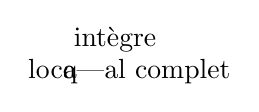
\begin{tikzpicture}[baseline=(base.base)]
\node[inner sep=0] (base) {loc\unsure{\rlap{q}a|a}l \uline{complet}};
\path (base.north west) -- coordinate[pos=.43] (ins) (base.north east);
\node[anchor=south,inner sep=0,yshift=.08cm] at (ins) {\inserted{intègre}};
\end{tikzpicture}}, donc unibranche, mais en l'occurrence non géométriquement unibranche, est donné par $\overset{\textstyle\inserted{A=}}{\text{\uuline{R}}}\ X,Y\quad/(X^{\handwritten{2}}+Y^{\handwritten{2}})$. \deleted{Si $X$ est son spectre} Alors $A\otimes_{\underline{R}}\underline{C}$ est étale sur $A$, mais non intègre. Ces exemples, qu'on semble rencontrer pour la première fois à propos de 6.15.7. pourraient peut-être remonter à cet endroit.\handwritten{/} Il est cependant p\rlap{o}lausible que \deleted{l'énoncé qui} la reponse à la question suivante soit affirmative :}

\deleted{Soit $A\quad B$ un homomorphisme local d'anneaux locaux noethériens, $B$ plat sur $A$, $B\otimes_A k\handwritten{/}k$ géométriquement intègre, $A$ \deleted{excellent (par exemple complet)} géométriquement unibranche (NB on peut se ramener au cas: $A$ normal). Si $A$ est de plus excellent (disons complet), alors $B$ est-il intègre ?}

\deleted{La reponse est affirmative quand le corps résiduel $k$ de $A$ est de car 0, comme on verra au N\textsuperscript{\uline{o}} 7.9. en utilisant la\deleted{é} résolution des singularités de Hironaka, ou lorsque $B$ est essentiellement de type fini sur $A$ (réf $\qquad$). M\rlap{i}a\rlap{a}is \mbox{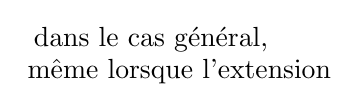
\begin{tikzpicture}[baseline=(base.base)]
\node[inner sep=0] (base) {même lorsque l'extension};
\node[anchor=south west,inner sep=0,yshift=.08cm,xshift=.08cm] at (base.north west) {\inserted{dans le cas général,}};
\end{tikzpicture}} résiduelle est triviale, $A$\deleted{\unsure{s|x}} et $B$ complet, \deleted{la technique \unsure{dévis}} nous ignorons si la réponse est affirmative. On a cependant un résultat partiel ci-dessous.}
